\subsection{第 13 课 | 字典树和并查集}

\subsubsection{脑图}

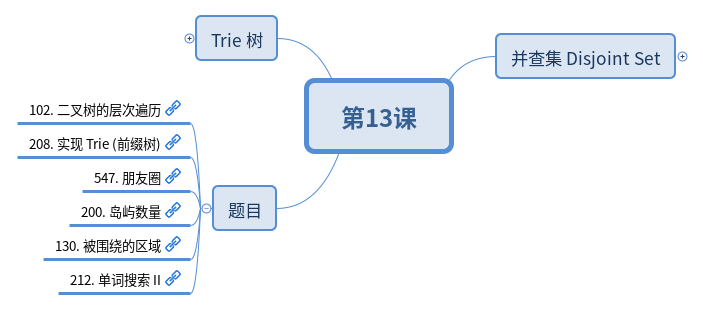
\includegraphics[width=140mm,height=60mm]{images/camp/第13课.png}

\subsubsection{题目}

\begin{itemize}
  \item \hyperref[leetcode:102]{102. 二叉树的层次遍历}
  \item \hyperref[leetcode:208]{208. 实现 Trie (前缀树)}
  \item \hyperref[leetcode:547]{547. 朋友圈}
  \item \hyperref[leetcode:200]{200. 岛屿数量}
  \item \hyperref[leetcode:130]{130. 被围绕的区域}
  \item \hyperref[leetcode:212]{212. 单词搜索 II}
\end{itemize}
